\documentclass{article}
\usepackage[utf8]{inputenc}
\usepackage{listings}
\usepackage{float}
\usepackage{natbib}
\usepackage{graphicx}
\usepackage{amssymb}
\usepackage{amsmath}
\title{Constellation}
\author{A blockchain microservice operating system}
\date{November 25 2017}
\setlength{\parskip}{1em}

 
\begin{document}

\maketitle

\begin{abstract}
Current blockchain technology such as Bitcoin, Ethereum, and others have systemic synchronous limitations that render them unsuited for mass adoption into the current technical architecture of distributed consumer applications. Consensus mechanisms and smart contract architecture cannot scale to a level that is required for consumer grade applications to function. We propose a fault resistant, horizontally scalable, distributed operating system that can implement full nodes as a mobile client. Therefore, we present a reformulation of cryptographically secure consensus into a modern server-less architecture using an asynchronous ExtendedTrustChain, Proof-of-Meme consensus model,  smart contracts as composeable microservices using the JVM and initially implemented as an actor based finite state machine. This architecture ensures high transaction throughput, allowing for consumer grade distributed applications to be built on Constellation. \

\end{abstract}
\setcounter{secnumdepth}{0}
\section{Introduction}
Despite the goal of decentralization, cryptocurrencies are operated and secured by increasingly centralized networks and mining organizations that control the security of the network\footnote{Digital Currency Group 'Bitcoin Scaling Agreement at Consensus 2017' medium.com/@DCGco}. With the rise of post Bitcoin networks such as Ethereum, the main goal of processing financial transactions has been expanded to provide trustless distributed computation by way of the EVM and its smart contract system of logic. While diverse and creative implementations of these distributed protocols exist, they are siloed from existing mainstream software and as such there is a high barrier to entry\footnote{J. Evans 'Blockchains are the new Linux, not the new internet' techcrunch.com}. This means that for businesses and enterprises that are looking to use blockchain technology it is highly costly and time intensive to develop and deploy scalable distributed applications. Therefore, requiring high levels of technical skill to execute and build well developed, bug-free distributed applications. To overcome these technical challenges blockchain technology requires a self-sustaining protocol that functions as a horizontally scalable, cost effective, and efficient distributed operating system.

Bitcoin was created to solve the problem of distributed consensus for financial transactions, but relied upon the energy intensive consensus process known as proof of work. This pools vertical computational power from a select few individuals with well-developed and hence centralized computing power\footnote{'Has Bitcoin Become Centralized?' www.trustnodes.com}. This puts network security and rewards into the hands of the same select few. As scaling debates have escalated for these parties it has led to the creation of several Bitcoin forks such as Bitcoin Cash and Bitcoin Gold these divided political factions are highly divisive and damaging to the ecosystem. Antiquated throughput requirements (i.e. capped 1MB block size) combined with a time intensive algorithm has caused transaction times and transaction fees to skyrocket. Ethereum uses a similar but ASIC-resistant proof-of-work consensus algorithm and is  moving to a proof-of-stake consensus mechanism, Casper.  With proof-of-stake there is a democratic imbalance where those with the most money get to choose the state of the network through consensus. Ethereum pioneered the use of smart contracts, however due to their synchronous execution consumer ready distributed applications are severely bottlenecked. Concurrency is key to providing consumer focused products and Constellation achieves this with its smart contract as microservice architecture.

\subsection{What makes Constellation different?}
The blockchain development community has been looking for new implementations of distributed ledger technology to solve the scalability issue and has so far failed to solve this. The problem still remains, how can we process more transactions and perform more services in less time with less cost? We propose a horizontal scaling approach that applies techniques similar to MapReduce.  

Horizontal scalability is the application of concurrent programming; it means that as users join the network, transaction throughput increases. MapReduce is a process of breaking computation into simple operations that can be fed into an asynchronous DAG (directed acyclic graph) of computation, thereby increasing the efficiency of an already concurrent program. 

The Constellation protocol implements a horizontally scalable blockchain architecture known as Extended Trust Chain with a peer to peer layer known as a gossip protocol that can be deployed on a native mobile device. Constellation approaches smart contracts with a microservice architecture allowing for highly available services to be chained and composed into distributed applications with just an understanding of each microservice's SLA's (service level agreement) and/or type signature.

Gossip protocols allow for large networks to communicate total network state at a scale that is orders of magnitude higher than existing blockchain technology\footnote{R. van Renesse 'A Blockchain Based on Gossip?' zurich.ibm.com}. In this network each member of the network keeps track of its neighbors and when it receives new messages, it propagates that message to all of its neighbors in turn. This has some interesting mathematical properties, but in our case, it allows for a large pool of connected devices to share the state of the network and achieve consensus at a scale that is unheard of on current blockchain implementations (see Figure 1).

\begin{figure}[H]
\centering
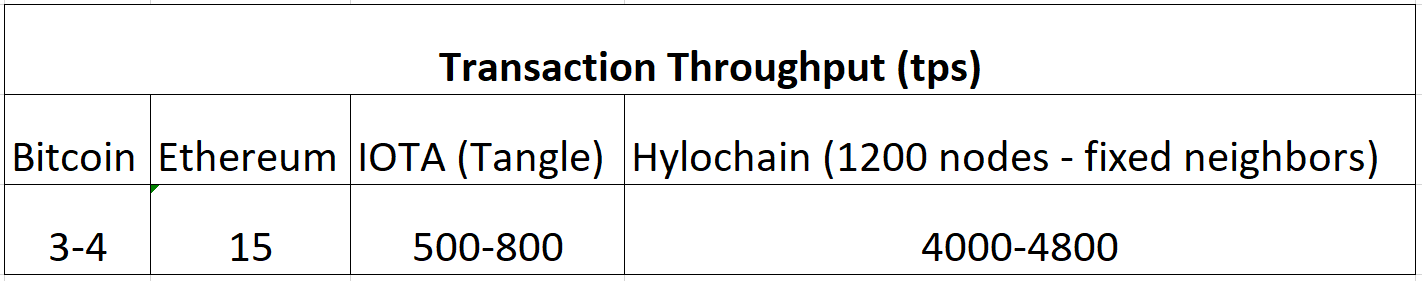
\includegraphics[scale=0.30]{Throughput.png}
\caption{Throughputs of comparable blockchains for comparison}
\end{figure} 

One approach to blockchain consensus that allows for horizontal scalability is ExtendedTrustChain. In ExtendedTrustChain, there are multiple node types, each with their own responsibility and role in the network asynchronously governing different aspects of the protocol. 

\begin{figure}[H]
\centering
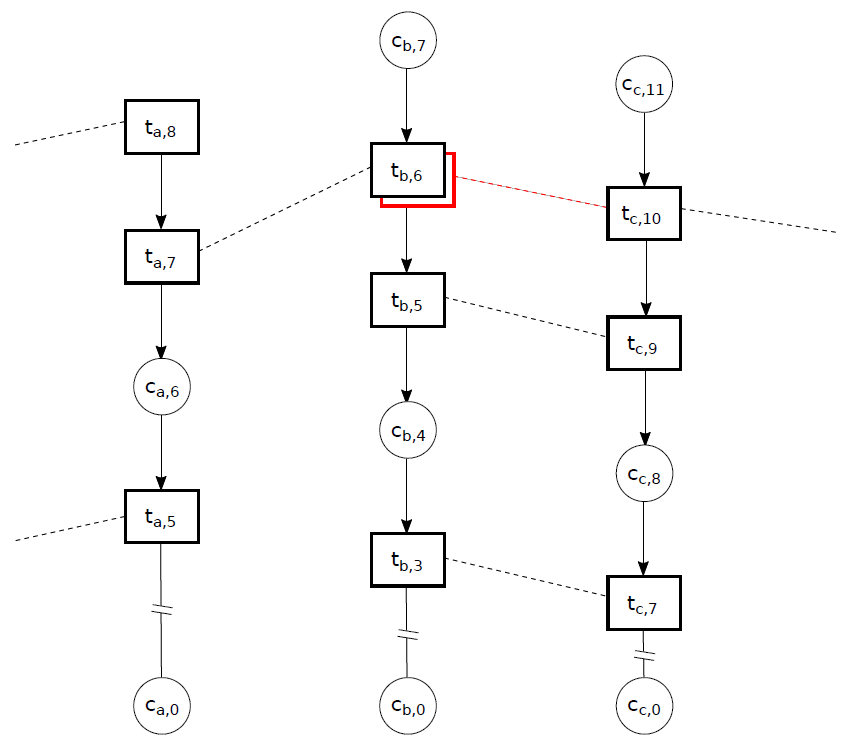
\includegraphics[scale=0.62]{kcong-extended-trust-chain.PNG}
\caption{Diagram of Extended Trust Chain, K. Cong et al.}
\end{figure} 

\subsection{Nodes}
Specifically, there are basic nodes that send transactions and hosts a member's individual chain (each individual's chain forms a DAG with others on the network when a transaction is made and is hashed into linear blocks). 

\subsection{Checkpoint Processes}
There are node processes that perform consensus on transactions (which fill a buffer and are hashed into checkpoint blocks), these collections of transactions will be hashed and become the next block in the main chain. 

\subsection{Validator Processes}
Finally, there are validator nodes which run validation processes and host the current chain state and hence seed the chain state/history to nodes on the network. 

\section{EVM vs JVM}
The formulation of distributed applications as MapReduce operations on smart contracts has been proposed by the Plasma upgrade to Ethereum\footnote{V. Buterin et al. \url{https://plasma.io/plasma.pdf}}. However, with its application to the EVM, it still suffers the same pitfalls of synchronous architecture for scaling in a cost effective and low-latency way. The Solidity programming language was built to address the risks of non-determinism in smart contract development. The need for deterministic instruction stems from the need to calculate the cost of running a Smart Contract and as a preventative measure against DDOS attacks, and messaging spam to the network. However, if compiled byte code could be notarized on chain and verified in a JVM, then deterministic compilation becomes a looser requirement\footnote{Corda}. Reduction in gas consumption, circumvention of gas limits and smart contracts with the complexity of microservices would then become a possibility.

It is logical to design distributed applications as compositions of successful building blocks, like assembling Legos where each piece is an existing microservice. Taking this one step further we implement on-chain interoperability which allows blockchain companies to provide distributed applications for reuse by others as building blocks for more complex distributed applications. A truly decentralized ecosystem cannot exist with monolithic smart contracts, thereby making this type of code ruse impossible and inefficient. 

The use of the JVM as a conduit for distributed applications is an industry standard in the Big Data community. Consumer applications are deployed as a collection of microservices on auto scaling groups which rely on easy provisioning, like the JVM provides. In these scenarios thousand node clusters can be provisioned and auto scaled on AWS virtual instances. The same scalability can be realized with Constellation's microservices architecture, which allows for the provisioning of resources as needed; thereby providing a dynamically scalable distributed application architecture. 

This type of distributed architecture inherently requires the modularity that functional programming provides. Therefore, we are using the Scala programming language to build an interface that can be implemented by any JVM language. When microservices are designed as concrete types, distributed applications can be composed of them directly in source code, allowing for validation at compile time. Developers can create new functionality by chaining together smart contracts of applicable types into composite applications; a constellation of computational logic is hence composed as one or more microservices or distributed applications. Constellation's smart contract interface will be designed with covariant and contravariant typing in mind, which mean that if we mix incompatible microservices or distributed applications, we will know immediately. Because of this we can even create constellations including smart contracts from other blockchains, pending solutions to cross chain liquidity issues like Polkadot\footnote{G. Wood et al. \url{https://github.com/w3f/polkadot-white-paper/raw/master/PolkaDotPaper.pdf}}.

Considering our functional programming ethos, it is worth noting that our consensus protocol could be described by the category theoretic definition of a hylomorphism.

\section{HyloChain - Conesus Architecture}
We have named our consensus architecture HyloChain because the underlying consensus architecture of Constellation is hylomorphic. A round of consensus takes the resulting hash block of a previous round and adds it as a regular transaction to the transaction pool. The filling of the transaction pool is isomorphic to an unfold operation. Once this checkpoint block is filled with the previous round plus new transactions it is hashed, this is isomorphic to a fold operation. 

\subsection{Definition: HyloChain}
A hylomorphism $h: A \rightarrow C$ can be defined in terms of its separate anamorphic and catamorphic parts. Take the definition of a hylomorphism

\begin{equation}
h = [(c, \oplus),(g, p)]
\end{equation}

The anamorphic part can be defined in terms of a unary function $g: A \rightarrow B \bigtimes A$ defining the list of elements in $B$ via repeated application or unfolding, and a predicate  $p:A \rightarrow \text{Boolean}}$  providing the terminating condition.

The catamorphic part can be defined as a combination of an initial value $ c \in C$ for the fold and a binary operator $ \oplus :B \times C\rightarrow C$ used to perform a fold. In our case the gossiping of messages is our anamorphism and the hashing of those messages plus the result of the previous block is our catamorphism.

If an operator is defined as a cryptographic hash function, $ \oplus = \text{CHash}$ and $g\ n=(n,n-1)$ and $p\ n = \text{False}$ (as our chain has no termination condition) for the nth iteration, HyloChain is defined categorically as 

\begin{equation}
HyloChain = [( \text{GenesisBlock}, \oplus),(g, p)]
\end{equation}

where GenesisBlock is our starting element, namely the genesis block used when we deploy HyloChain.

\subsection{Relation to ExtendedTrustChain}
Our consensus architecture, HyloChain builds upon the ExtendedTrustChain architecture and expands upon it in the following ways. In ExtendedTrustChain, each node operates as an account, maintains the history of its own chain, and relies upon transaction order for validity (similar to HashGraph\footnote{ L BAIRD et al. \url{http://www.swirlds.com/downloads/SWIRLDS-TR-2016-01.pdf}} ). Transactions are signed by the initiator and counterparty then broadcasted to the network (via gossip). Delegates perform consensus on the transactions within a checkpoint block, are chosen based on their reputation. The consensus result is broadcasted again and added as a normal transaction to the next block. \footnote{Kelong Cong, et al. https://repository.tudelft.nl/islandora/object/uuid:86b2d4d8-642e-4d0f-8fc7-d7a2e331e0e9?collection=education}

\begin{figure}[H]
\centering
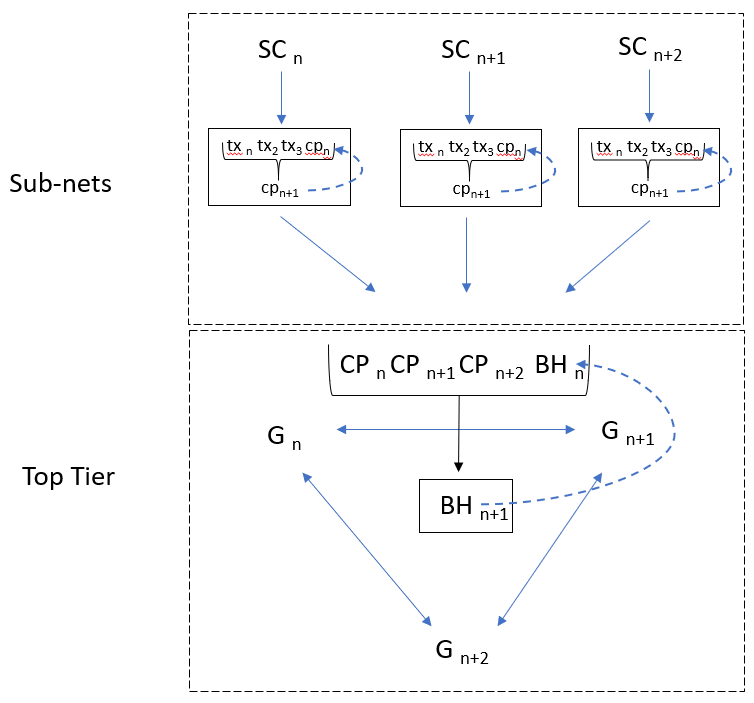
\includegraphics[scale=0.65]{HyloChain.png}
\caption{HyloChain}
\end{figure} 

\subsection{Fault Tolerance}
The fault tolerance of Contellation's HyloChain follows a typical Byzantine consensus model. The probability of an adversary taking control of network consensus approaches 1/2 as its control of consensus participants approaches 1/3\footnote{M. Pease, R. Shostak and L. Lamport, ?Reaching agreement in the presence of faults?, Journal of the ACM (JACM), vol. 27, no. 2}. To ensure the security of the network we can use these bounds to pick specific parameters to tune fault tolerance while maximizing transaction throughput and reducing latency. 

\begin{figure}[H]
\centering
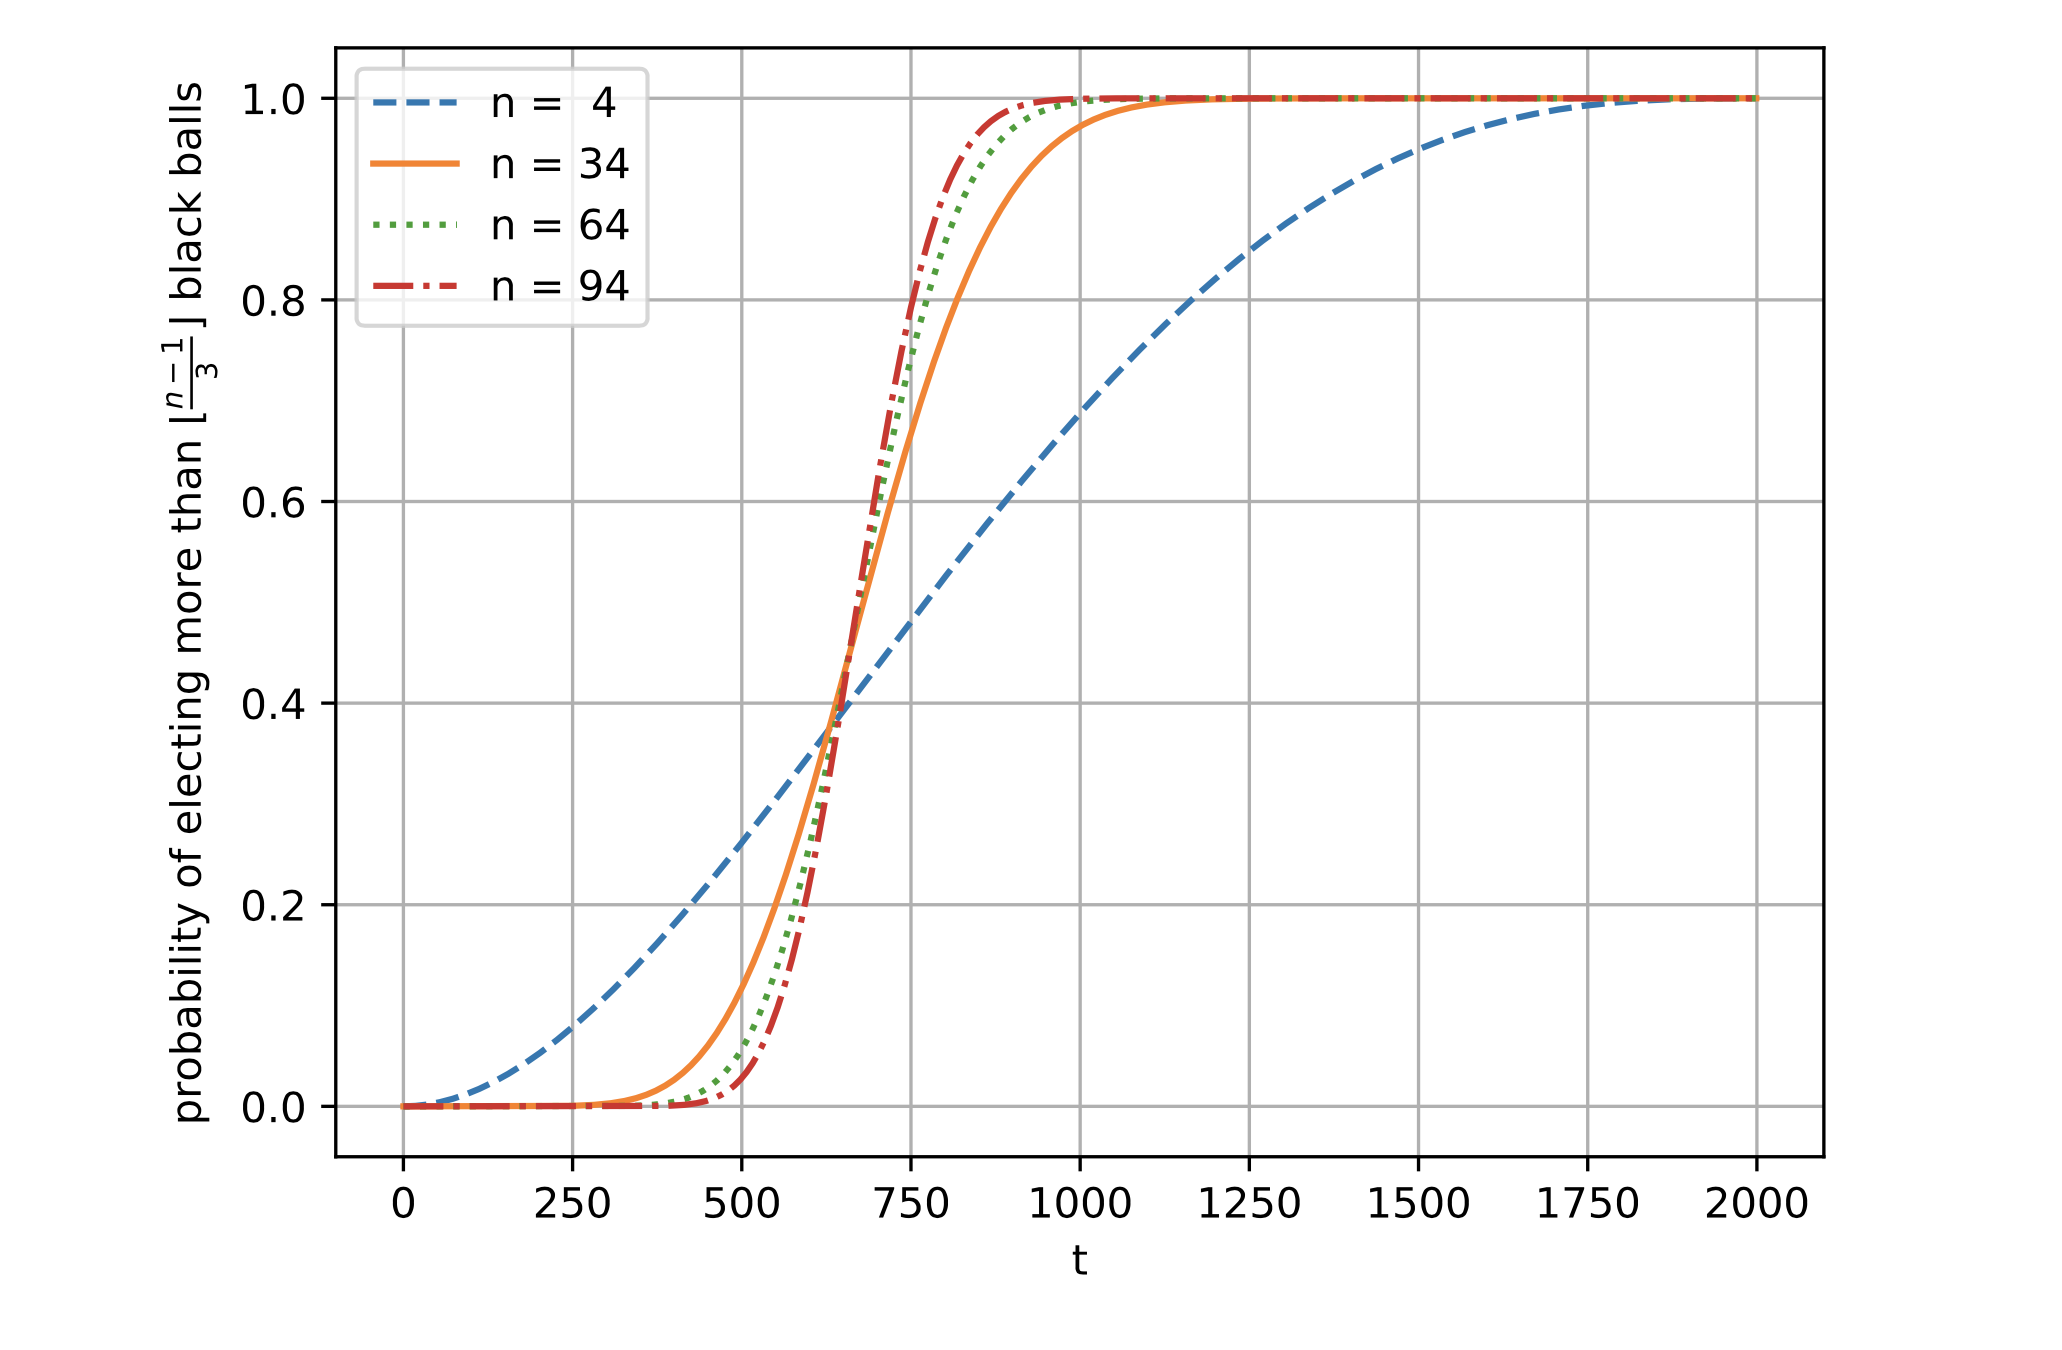
\includegraphics[scale=0.35]{fault-threshold-vs-byz-delegates.PNG}
\caption{Probability of selecting more than $(n-1)/3$ (denoted as black balls as this comes from an explanation of a hypergeometric distribution) for different values of $t$ (where t is the number of byzantine actors) with a population size fixed at 2000, K. Cong et al.}
\end{figure} 

Also, based upon our Byzantine consensus procedure (we are using Honeybadger BFT tentatively) and the double signing of transactions, it is impossible to fork the network. The only result of an incorrect consensus would be the censorship of individual transactions from a checkpoint block i.e a transaction lost during consensus. This would not cause loss of capitol and mitigation is as simple as resending to the network.

The relationship of throughput is linear with respect to the number of participants given the ability to horizontally scale, yet a linear increase in fault tolerance costs a polynomial increase in communication cost\footnote{pp 50, K. Cong, et al.}. Thus, we must determine consensus parameters that ensure maximum throughput with bounded fault tolerance and transaction confirmation time. How are we to scale a network with such bounds? Our approach is to compose our network's blockchain as a hierarchy of sub nets (Figure 1), each performing their own consensus, the results of which are bubbled up to a higher tier that processes these checkpoint bocks as ordinary transactions. This approach is very similar to Chain Fibers (also in the use of validators) however, in that we apply the dimensionality reduction technique of locality sensitive hashing to increase the size of the transaction pool. Since the effect of this architecture is to reduce the complexity of consensus from an average case  of $O(n^3)$ or quadratic per node, using the fact that in Honeybadger BFT the consensus algorithm can be reduced to $O(1)$ per delegate\footnote{A. Miller, Y. Xia, K. Croman, E. Shi and D. Song, ?The honey badger of bft protocols?, in Proceedings of the 2016 ACM SIGSAC Conference on Com- puter and Communications Security, ACM, 2016}, our complexity becomes

\begin{equation}
O(n) \rightarrow O(m) : m<<n
\end{equation}

Thus this is sub-linear with respect to the number of nodes in the sub net. 

In this case we refer to these checkpoint blocks as locality sensitive hash blocks. Each sub-net forms a locality sensitive block hash and sends it to the parent net (Galaxies, described below). This parent net then treats locality sensitive block hashes as ordinary transactions in the next round of consensus. To increase the performance of the network the choice of neighbors in a sub net need only depend on minimization of latency, as each node keeps track of its own transaction history.

In each level of scale, the same self-similar architecture of gossiped message passing is employed, allowing for the same nodes to participate at each level with only a change in resources provided by nodes.

All nodes in Constellation can be  "sleepy" i.e. they can join and leave the network at any time. As new nodes join the network, their resources are allocated to a sub-net. Once the sub-net reaches the threshold for transaction throughput and cryptographic security (the number of facilitators vs. the number of participants) as outlined above, entering nodes must form a new sub-net . Thus, new sub-nets will be dynamically allocated as members leave and join the network. The goal of this self-similar structure and our delegate selection model outlined below is to enable dynamic auto scaling based on network resources, allowing for consistent throughput. It is trivial to show that this architecture exhibits the power law intrinsic of scale-free networks which are notorious for their application to fault tolerance in complex systems such as distributed computing\footnote{}. 

\begin{figure}[H]
\centering
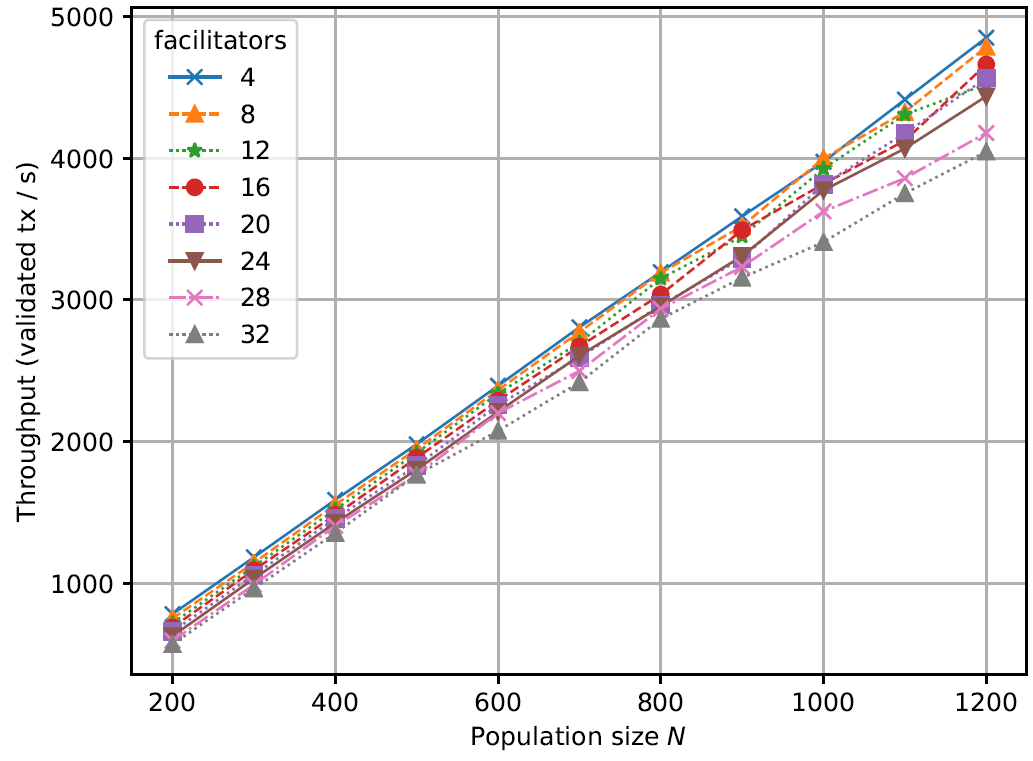
\includegraphics[scale=0.45]{hylochain-throughput-graph}
\caption{HyloChain throughput vs population, K. Cong et al.}
\end{figure} 

\section{Delegate selection model: Proof-of-Meme}
Fault tolerance in TrustChains can be improved with a reputation system for selecting delegates \footnote{pp 50, K. Cong, et al.}. We, therefore, present Proof-of-Meme; a deterministic mathematical model that scores a node's historical participation in the network. This model is used to determine the probability of a node being chosen to participate in consensus as a probability distribution. Our use of reputation based scoring and delegate selection such as Proof-of-Meme, in conjunction with each node's role as an individual account, allows our permissionless network the benefits of a permissioned system.

A meme in our sense is a feature vector corresponding to each node's account, in the simplest case an array of float values used as input to a deterministic machine learning algorithm. Each feature is representative of a node's utility to the network (has it been notable faulty during consensus, how much memory can it commit to consensus and so on and so forth). A meme can be transformed into a numeric value by passing it into a function, a to-be-trained model as described above, which is how we will quantify a meme's reputation. In order to provide a mechanism that promotes new nodes to improve their meme, a probability distribution of meme scores is drawn over buckets of fixed size; the distribution outlines the probability that a meme of a score in a particular bucket gets selected. This is meant to maximize throughput by relaxing the number of facilitators yet maintaining the same level of fault tolerance and confirmation times. Reputable memes will be given preference, but new memes will also have an opportunity to participate and build their reputation on the network. Logs of performance will be notarized on chain, so memes that provide faulty resources or perform in an adversarial way will have their reputation reduced while high performing and trustworthy memes will have theirs increased. Our idea for delegate selection in the inductive case is as follows:

1)	Consensus is performed.

2)	The hash block is fed to a deterministic algorithm that outputs updated meme scores for each delegate. This is performed at the top consensus tier (Galaxy) which is responsible for choosing facilitators.

3)	This constant is used to shuffle our distribution (move memes between buckets based on new data of their performance).

4)	The previous block hash (result of last consensus) is used to sort the contents of each bucket and the top N from each bucket (according to a probability distribution) are selected for this round. The meme of a consensus participant who acts faulty or provably malicious (as verifiable within logs) will be docked in the next consensus participant election.

As meme reputation begins to hold more value, it replaces the need for a transaction fee. Microservices may look to reputable memes for service hosting, which would be more profitable than earning transaction fees for performing consensus. Instead of increasing prices when latency is high, memes with low reputation scores will be throttled; their transactions processed with lower priority. A meme in this case would provision resources (participate in consensus), thus increasing throughput for themselves and solving bandwidth issues for the network.

 \subsection{Own your meme}
Constellation will not have network transaction fees rather, reputation will be our mechanism for preventing latency and adversarial attacks. In order to seed our network, a network incentive will be provided in the form of newly minted tokens after the initial genesis block (which will allocate tokens for ICO participants) with diminishing returns up until a fixed date. Newly minted tokens will be allocated based upon their each meme's reputation.

Consider the scenario of a point of sale system, specifically a vending machine. A vending machine that runs on Constellation could be implemented as a microservice that elects to participate in consensus. It's meme's reputation will grow over time and short transaction times would be ensured even in high traffic situations. This is vital as a real-world application needs high throughput in order to provide a competitive service. This means that even if a vending machine patron has a low meme reputation, the high reputation of the vending machine ensures that the patron will receive their item expediently even in a high traffic period. 

\section{Peer to Peer Architecture}
Our previous sections touch on the architecture of our peer to peer layer and it shall now be detailed. 

\subsection{Stars}
A Star is the base object in constellation. To interact directly with the network, users instantiate a star node on a device and transactions are issued through this Star instance. Each Star contains a local chain that is composed of its history on the network. This local chain is used to enforce ordering and is identified by the public key, who's private counterpart is used to sign transactions. A Star itself is a lightweight client for a user to interact with the network and is natively compatible with mobile devices. However, if a star wishes, it can elect to participate in consensus, which will allow it to appreciate its meme's reputation. If a star elects to participate in consensus, then it joins a collection of stars, which we refer to as a Star Cluster.

\subsection{Star Clusters}
A Star Cluster is a collection of Stars who have elected to participate in consensus. The total number of stars is limited by an upper bound, which will be determined after sufficient experimental and statistical analysis as outlined above  . When we reach this threshold, a new Star Cluster is created and each one of them forms locality sensitive hash blocks. These locality sensitive hash blocks are then treated like ordinary transactions and hashed by Galaxies into, namely Black Holes.

\subsection{Galaxies}
Galaxies are isomorphic to the role of validators in the ExtendedTrustChain yet they also serve as an auto scaling group, provisioning resources for new Star Clusters and maintaining meme reputation. Meme reputation is calculated by looking at logs of consensus performance. Metadata about the contents of a block proposed, latency, and failure are sent with locality sensitive hash blocks to Galaxies. Once Galaxies receive that data, meme reputations are updated before a new sample is chosen for the next round of consensus. Galaxies, as they are validators, provide a source of truth for removing invalid transactions and decide delegates in Star Clusters. Metadata about Galaxy performance is stored in Black Holes. As Stars build reach a threshold of reputation, they may earn the right to function as Galaxy nodes.

\subsection{Black Holes}
Black Holes are blocks of hashed locality sensitive hash blocks. It is equivalent to refer to them as blocks in the block chain. Galaxies store the full history of the blockchain.

\section{Smart contracts as microservices}
Highly available, elastic, distributed systems thrive on a server less architecture. In the case of a distributed operating system this can be achieved as a network of distributed microservices. Thus, in constellation, smart contracts themselves are microservices running on a JVM. They can send transactions, sign as a counterparty and perform consensus. The goal is for the microservices themselves to operate as a Star with a corresponding meme, providing services for agreed upon amounts. They can serve the same role as smart contracts in Ethereum or Counterparty, but in addition provide more complex logic by utilizing the existing codebase in the JVM ecosystem. In addition, they can talk to external programs through an RPC interface. If these microservices are built with concrete service level agreements or better yet, type signature, their composite logic can be chained and composed into distributed applications intuitively. This is where MapReduce operators come into play. A smart contract microservice can be designed to send and receive data models that improve computational complexity (given our asynchronous architecture) and can be repurposed for new applications.

Considering the celestial metaphor above, it is worth noting that distributed applications on Constellation are constellations themselves. As each microservice is a  Star, collections of microservices chained and/or composed can be connected by a line that represents an application. It is trivial to notice that when drawn, this produces a constellation.

\section{Constellation as a Blockchain Operating System}
The above server less architecture is an instance of a distributed operating system. The goal of an operating system is to provide an interface for the utilization of underlying hardware's resources. This is integral for application development, allowing for high level programming languages and intuitive user interfaces. A distributed operating system differs in that it aims to provide an interface for the underlying resources of a distributed compute cluster. As blockchains are inherently a distributed system, writing blockchain compatible applications requires a distributed operating system in order to utilize the full power of the underlying cluster. Typically, operating systems require a program that maintains the underlying hardware state, this is called a kernel. It's possible to construct a distributed operating system with a serverless architecture  . In our scenario as in MicroOs, the operating system is a collection of microservices. Extrapolating this, from the perspective of an application developer, microservices are the building blocks, much like Legos, for comprehensive applications built with Constellation. The goal of this is to allow even non-technical individuals to construct applications using existing microservices as building blocks. This coupled with an intuitive user interface provides a frictionless on-ramp for non-technical users to develop distributed applications on Constellation.

As we have described above, the ability of an individual to seamlessly (non-technically) materialize an idea into an application, one could say that this is the  transmutation of potential energy from the Noosphere into the material world. Because of this, we have decided to name our currency noOs, in light of the noospheric potential energy that makes up our goals and ideas.

\subsection{Conclusion}
We presented a reformulation of cryptographically secure consensus into modern serverless architecture that will allow mainstream applications to use blockchain technology. Our approach applied the dimensionality reduction technique of locality sensitive hashing as a divide and conquer mechanism allowing for a Trust Chain at internet scale. Our meme economy provides a deeper layer of cryptographic security and the potential to make transaction fees obsolete. In addition, we provide an intuitive celestial metaphor for our distributed architecture and draw an intuitive correlation between distributed applications and why we chose to name this protocol Constellation.

\bibliographystyle{plain}
\end{document}
